  \documentclass[14pt, oneside]{book}
    \usepackage[margin=1in]{geometry} 
    \usepackage[brazilian]{babel}
    \usepackage{graphicx}
    \usepackage[utf8]{inputenc}
    \usepackage[T1]{fontenc}
    \usepackage{amsmath,amsthm,amssymb,amsfonts, physics}
    \usepackage{enumitem, verbatim}
    \usepackage{multicol}
    \usepackage{mathtools}
    \usepackage{titlesec}
    \usepackage{indentfirst}
    \renewcommand{\baselinestretch}{1.5}
    \usepackage{hyperref, color}
    \usepackage{float}
    \usepackage[nottoc,numbib]{tocbibind}
        \hypersetup{
            colorlinks=false, %set true if you want colored links
            linktoc=all,     %set to all if you want both sections and subsections linked
            linkcolor=blue,  %choose some color if you want links to stand out
        }
    \usepackage{listings}
    \titleformat{\chapter}[hang]{\bf\huge}{\thechapter}{2pc}{}
    \DeclarePairedDelimiter{\ceil}{\lceil}{\rceil}
    \date{\vspace{-5ex}}
    \lstset{language=Python}  
    \usepackage{pythonhighlight}
     
    \newcommand{\N}{\mathbb{N}}
    \newcommand{\Z}{\mathbb{Z}}
    \newcommand\tab[1][1cm]{\hspace*{#1}}
    \renewcommand{\qedsymbol}{$\blacksquare$}

%detalhes do projeto
%empresa 1 e empresa dois são empresas de design com parametros diferentes
%empresa 3 é uma empresa de construção civil

     
    
\theoremstyle{definition}
    \newtheorem{problem}{Problema}
    \newtheorem{dica}{Dica}
    \newtheorem{gabarito}{Gabarito}
    \newtheorem{defn}{Definição}
    \newtheorem{teorema}{Teorema}
    
\begin{document}
    \pagenumbering{gobble}

    \begin{titlepage}
        \centering 
        
\includegraphics[scale = 0.8]{ufpe.png} \\
        \Large{\textbf{UNIVERSIDADE FEDERAL DE PERNAMBUCO}}\\
        \large{Departamento de Eletrônica e Sistemas}
        \vspace*{\stretch{2.0}}
   
        \Huge\textbf{Sistemas de Controle}\\
        \Large\textbf{Sistema de Otimização de Recursos Humanos}
   
        \vspace*{\stretch{2.0}}
        \vfill
        \Large{Turma de Sistemas de Controle 2019.1} \\
        
        \Large{Maio, 2019}
    \end{titlepage}
\tableofcontents
\addtocontents{toc}{\protect\hypertarget{toc}{}}
\mainmatter
            \chapter[Motivação]{\hyperlink{toc}{Motivação}}
    A consumação de qualquer projeto real exige diversas etapas fundamentais para seu cumprimento, que transitam desde o planejamento, até a execução e o fechamento do mesmo. Sendo assim, os projetos são caracterizados por um tempo finito de envolvimento de profissionais responsáveis por diferentes funções em cada uma das etapas de desenvolvimento. O gerenciamento eficiente desses recursos humanos, são essenciais para garantir o correto andamento de projetos de maior complexidade, o que muitas vezes demanda uma abordagem matemática para garantir um bom processo gerencial.\\
            
     O presente projeto tem como objetivo permitir a visualização e análise de possíveis projeções sob condições reais da aplicação do método de otimização de recursos humanos, se utilizando da linguagem de programação Python. \textbf{A abordagem foi baseada no trabalho de conclusão de curso de Guilherme Cerqueira}. Tal metódo permite uma melhor e mais eficiente organização do potencial humano para o desenvolvimento de um trabalho em uma empresa.\\ %Melhorar a citação ao trabalho de Guilherme.
             
    
    O princípio do máximo de Pontryagin (PMP), princípio importantíssimo no estudo de sistemas de controle dinâmicos, é uma ferramenta para resolver problemas de maximização de funções sujeita a restrições:
            $$\text{Max }\int_{x_1}^{x_2}I(x,u,t)dt$$
             sujeito a:
            $$\frac{dx}{dt}=f(x,u,t)$$
             Tomando a condição dada, o PMP é resolvido utilizando uma função chamada função Hamiltoniana, definida como:
            $$H(x,u,t,y) = I(x,u,t) + y^Tf(x,u,t)$$
             Sendo assim, para encontrar a força de controle $u$ ótima, chamada de $u^\star$, segue-se o procedimento:
            $$\frac{\partial H}{\partial u^\star} = 0$$
            $$\frac{\partial H}{\partial u^\star} = \frac{dx}{dt}$$
            $$\frac{\partial H}{\partial u^\star} = -\frac{dy}{dt}$$
            
    A força de controle ótima, $u*$, deste estudo se baseia na política de contratação e demissão de profissionais em cada momento do projeto de forma a minimizar os custos. Matematicamente, o problema de minimização de uma função objetivo qualquer em nada se diferencia do problema de maximizar o negativo da mesma. A completa modelagem do problema será discutida na seção Modelagem, enquanto os resultados obtidos serão avaliados na seção Simulação.
    
    
            
            
            
            \chapter[Modelagem]{\hyperlink{toc}{Modelagem}}
      
            O objetivo deste trabalho, como adiantado anteriormente, é verificar a validade do modelo proposto de maneira teórica, expondo o Princípio de Máximo de Pontryangin ao escrutínio. Usou-se, portanto, o gerenciamento de funcionários responsáveis por um determinado projeto de uma companhia de grande porte qualquer como meio de estudo. Note-se, entretanto, que a demanda por funcionários é para um projeto específico, o que denota a sazonalidade da própria demanda. Devido às incertezas associadas ao gerenciamento de pessoas, a rotação de funcionarios é constante, ou seja, os números de funcionários demitidos e contratados seguem uma tendência a serem constantes. Por conta disso, a empresa deve controlar este problema, contratando novos funcionários e treinando-os ao longo do projeto. Assim, o modelo empregado neste trabalho leva em consideração que existem momentos de contratação e momentos de demissão, quando as respectivas práticas predominam, dependendo da fase em que o projeto se encontra. Ainda, é importante destacar que as variáveis detectam valores reais ao longo do tempo, o que as torna contínuas. 
            
             As variáveis utilizadas estão organizadas da seguinte maneira: \textbf{u} (variável de controle) como sendo a política de contratação/demissão, expressa em número de funcionários; \textbf{x\textsubscript{1}} (variável de estados) como o número de trabalhadores no projeto e \textbf{x\textsubscript{2}} (variável de estado) como o progresso do projeto de maneira percentual (de 0\% concluído até 100\% concluído). É importante que se tenha conhecimento acerca das limitações de cada variável, de maneira que resultados absurdos sejam eliminados do conjunto de soluções candidatas a soluções ótimas. Desta maneira, coloca-se as seguites restrições: a variável de controle \textbf{u} não possui quaisquer restrições, já que representa a quantidade de profissionais a serem contratados ou demitidos em determinada etapa do projeto; a variável de estado \textbf{x\textsubscript{1}} está restrita ao subconjunto [0,1] por representar uma porcentagem; e, por último, a variável de estado \textbf{x\textsubscript{2}} está limitada ao subconjunto dos reais positivos, inlcuindo o zero, já que é logicamente impossível ter um número negativo de funcionários trabalhando em um projeto.
             
            O custo total durante o tempo de execução do projeto será obtido a partir do custo com os funcionários presentes durante cada momento, e dos custos com contratação e demissão de outros profissionais ao longo do tempo. O que pode ser representado a partir da função objetivo:
            
            $$J\left(\eta,\xi \right) = \int_{\xi}^{\eta}\left[{\beta x_1 + \theta u^2}\right]dt$$
            
            Na qual o parâmetro $\beta$ foi considerado como o custo com pagamentos e encargos, enquanto o parâmetro $\theta$ representa o custo com contratações e demissões de funcionários. Deseja-se minimizar, portanto, o funcional objetivo $J\left(\eta,\xi \right)$ desde o início do projeto (tempo 0), até o tempo de término $\tau$. Levando-se em consideração também as equações dinâmicas das restrições, o modelo geral a ser resolvido será:
            
            $$\text{Min} -J\left(\eta,\xi \right) =- \int_{\xi}^{\eta}\left[{\beta x_1 + \theta u^2}\right]dt$$
            
            sujeito a:
            
            \begin{center}
            $\dot{x}_1 = u - \mu x_1$
            
            $\dot{x}_2 = \gamma x_1 - \alpha x_2$
            
            \end{center}
           
             Para garantir a coerência do modelo com o caso real outros parâmetros foram introduzidos nas equações dinâmicas de restrição, dentre eles o $\mu$, $\gamma$ e $\alpha$. O primeiro deles, $\mu$, é a taxa de rotatividade de funcionários no projeto, ou seja, indica a taxa com que os funcionários deixam o projeto ou são substituídos, seja por renúncia, acidentes de trabalho ou doenças. Portanto, a primeira equação dinâmica, $\dot{x}_1$, ilustra que a variação da equipe de trabalho em qualquer momento do projeto está relacionada com o quantitativo de funcionários contratados ou demitidos e o total de funcionários que abandonam o projeto. Para determinar $\mu$ um estudo detalhado das causas de abandono devem ser levados em consideração. O segundo parâmetro, $\gamma$, está relaciona relacionado com a produtividade da equipe, considerando uma performance homogênea dos membros. O terceiro parâmetro, $\alpha$, está relacionado com a dificuldade de finalização do projeto a medida que o mesmo é completado, i.e., a quantidade de retrabalho e dificuldades que podem surgir no andamento do projeto. Assim, a segunda equação dinâmica, $\dot{x}_2$, ilustra que a variação do andamento do projeto leva em cosideração a performance da equipe e as dificuldades inerentes à execução do projeto, bem como fatores externos que solicitam mudanças.
            
             Para resolver o problema de otimização proposto, usa-se a função chamada de Hamiltoniano, de onde as condições de otimalidade podem ser derivadas quando se aplica o Princípio de Máximo de Pontryagin. O Hamiltoniano segue:
            
            \begin{center}
                $H(x_1,x_2,u,y_1,y_2) = -\left[\beta x_1 + \theta u^2 \right] + y_1\left[u - \mu x_1 \right] + y_2\left[\gamma x_1 - \alpha x_2 \right]$
            \end{center}
            
             Ainda, as equações propostas pelo Princípio de Máximo de Pontryagin seguem abaixo:
            
            \begin{center}
                $\frac{\partial H}{\partial u} = 2\theta u + y_1 = 0$
                
                $\frac{\partial H}{\partial x_1} = -\dot{x_1} = -\beta - \mu y_1 + \gamma y_2$
                
                $\frac{\partial H}{\partial x_2} = -\dot{y_2} = -\alpha y_2$
                
                $\frac{\partial H}{\partial y_1} = \dot{x_1} = u-\mu x_1$
                
                $\frac{\partial H}{\partial y_2} = \dot{x_2} = \gamma x_1 - \alpha x_2$
            \end{center}
            
            As soluções das equações acima são dadas abaixo:
            
            \begin{center}
                $u = -\frac{\beta}{2\theta \mu} - \frac{\gamma A e^{\alpha t}}{2\theta (\alpha - \mu)} + \frac{B e^{\mu t}}{2\theta}$
                
                $x_1 = -\frac{\beta}{2\theta \mu^2} - \frac{\gamma A e^{\alpha t}}{2\theta (\alpha^2 - \mu^2)} + \frac{Be^{\mu t}}{4\theta \mu} - Ce^{-\mu t}$
                
                $x_2 = -\frac{\gamma \beta}{2\theta \alpha \mu^2} - \frac{\gamma^2 Ae^{\alpha t}}{4\theta \alpha (\alpha^2 - \mu^2)} + \frac{\gamma Be^{\mu t}}{4\theta \mu (\alpha + \mu)} \frac{-\gamma Ce^{-\mu t}}{(\alpha - \mu)} + De^{-\alpha t}$
            \end{center}
            
            Para as condições iniciais, levar-se-á em conta que
            \begin{center}
            $\dot{x_2} \geq 0$ \implies $\gamma x_1(t) - \alpha x_2(t) = 0$    
            \end{center}
            
            Esta relação impede a evolução negativa de um projeto, dada uma sequência de atividades até sua conclusão. Portanto, para quaisquer condições iniciais e finais, ter-se-á certeza acerca do cumprimento do projeto. Por exemplo, a empresa pode iniciar o projeto sem funcionários e, ainda assim, completá-lo de maneira ótima.
            
            \chapter[Simulação]{\hyperlink{toc}{Simulação}}
            O código realizado em \textit{python} resolve as variáveis de integrações levando em conta a arbitração dos parâmetros: $\alpha, \mu, \gamma, \beta, \theta$ e $\tau$. Os valores considerados levaram em conta o custo total da obra, o número de funcionários e tempo de execução.
            
            A partir desses parâmetros foram calculados os valores para $u$, $x_1$ e $x_2$ para em seguida serem plotados os gráficos. Os dados utilizados foram retirados de duas empresas de \textit{desing} e uma de construção civil. Alguns pontos devem ser considerados para esses dados e os valores dos parâmetros, primeiramente, o número de funcionários de uma empresa de \textit{design} é muito menor que o de uma construção civil, além disso, eles tem um maior impacto na produto final, ou seja, a sua produtividade é maior, por isso o $\gamma$ de uma empresa desse tipo é maior que o de uma construção.
            
            Os gráficos das Figuras \ref{empresa1_u}, \ref{empresa2_u} e \ref{empresa3_u} mostram o número de contratações/demissões de funcionários e observando seu formato nota-se que está de acordo com a teoria estudada, pois no início de um projeto precisa-se contratar os trabalhadores, enquanto que no final é necessário demití-los devido ao fim da obra.
            
            As Figuras \ref{empresa1_n}, \ref{empresa2_n} e \ref{empresa3_n} são os gráficos trapezoidais, que mostram a quantidade de pessoas no projeto de acordo com o tempo. No início, há uma crescente, pois precisa-se contratar trabalhadores, em seguida há uma estagnação que significa que a obra está em andamento e ,perto do fm, começa-se a demitir funcionários devido ao fim da obra.
            
            Note-se, contudo, que, mesmo quando o término do projeto se aproxima, a quantidade de trabalhadores não fica abaixo de uma quantidade mínima em nenhum dos casos apresentados nas figuras abaixo. Isso ocorre porque existe uma possibilidade do projeto retornar a uma etapa indesejada e, portanto, necessitar-se-ia de mão-de-obra de emergência.
           
            Por fim, as Figuras \ref{empresa1_p}, \ref{empresa2_p} e \ref{empresa3_p} representam o andamento da obra em percentagem. Como pode-se observar, todas elas estão em "formato de s" significando que a produtividade está no máximo.
            
            \begin{figure}[H]
                \centering
                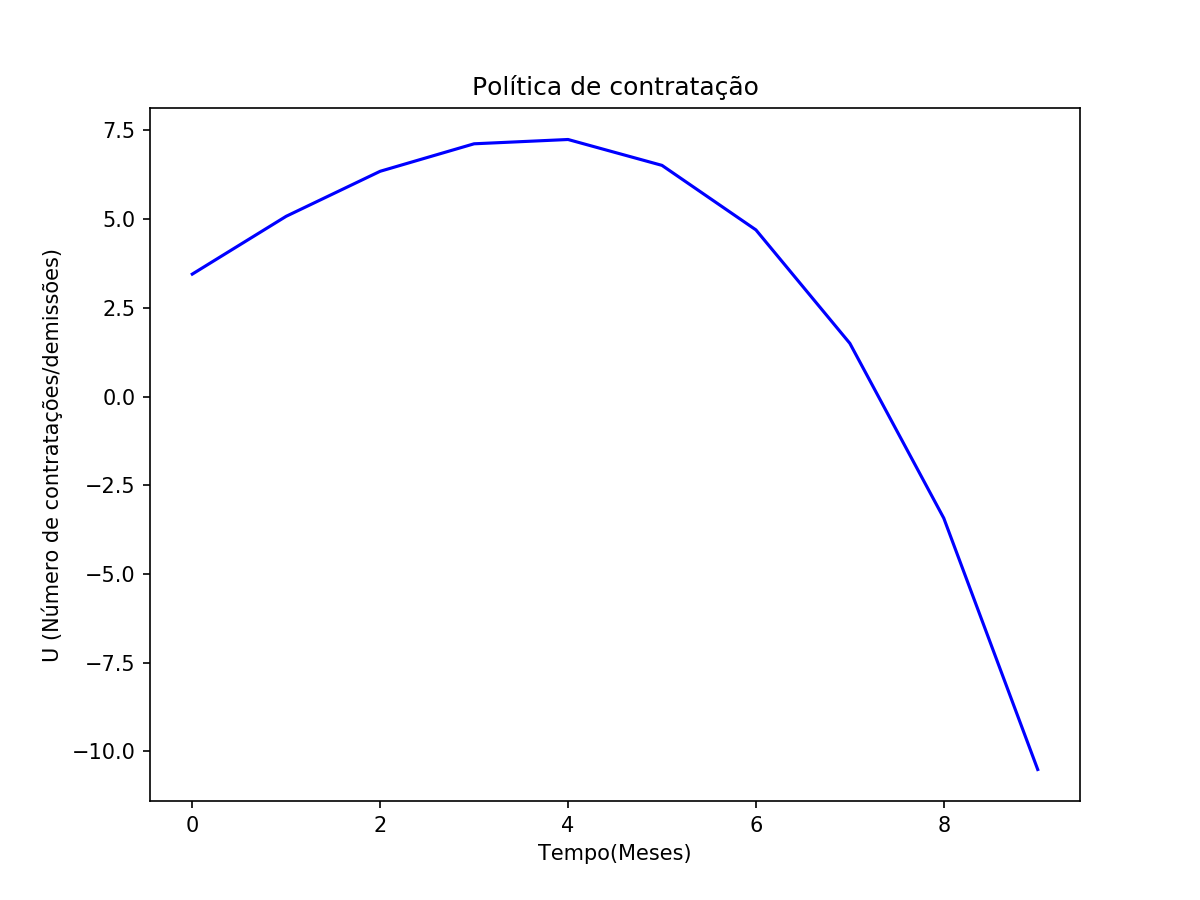
\includegraphics[scale=0.9]{empresa1_u.png}
                \caption{Número de Contratações do Projeto 1}
                \label{empresa1_u}
            \end{figure}
            
            \begin{figure}[H]
                \centering
                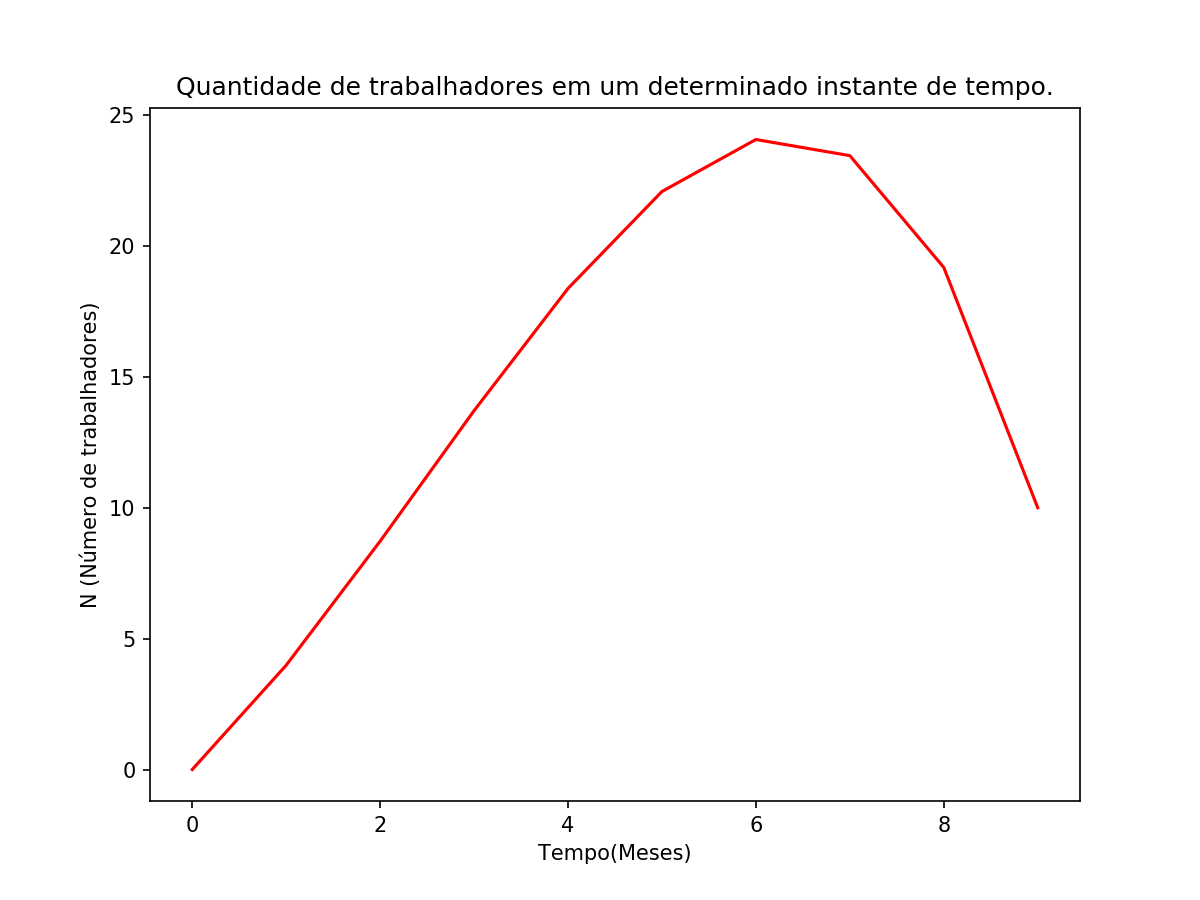
\includegraphics[scale=0.9]{empresa1_n.png}
                \caption{Número de Funcionários do Projeto 1}
                \label{empresa1_n}
            \end{figure}
            
            \begin{figure}[H]
                \centering
                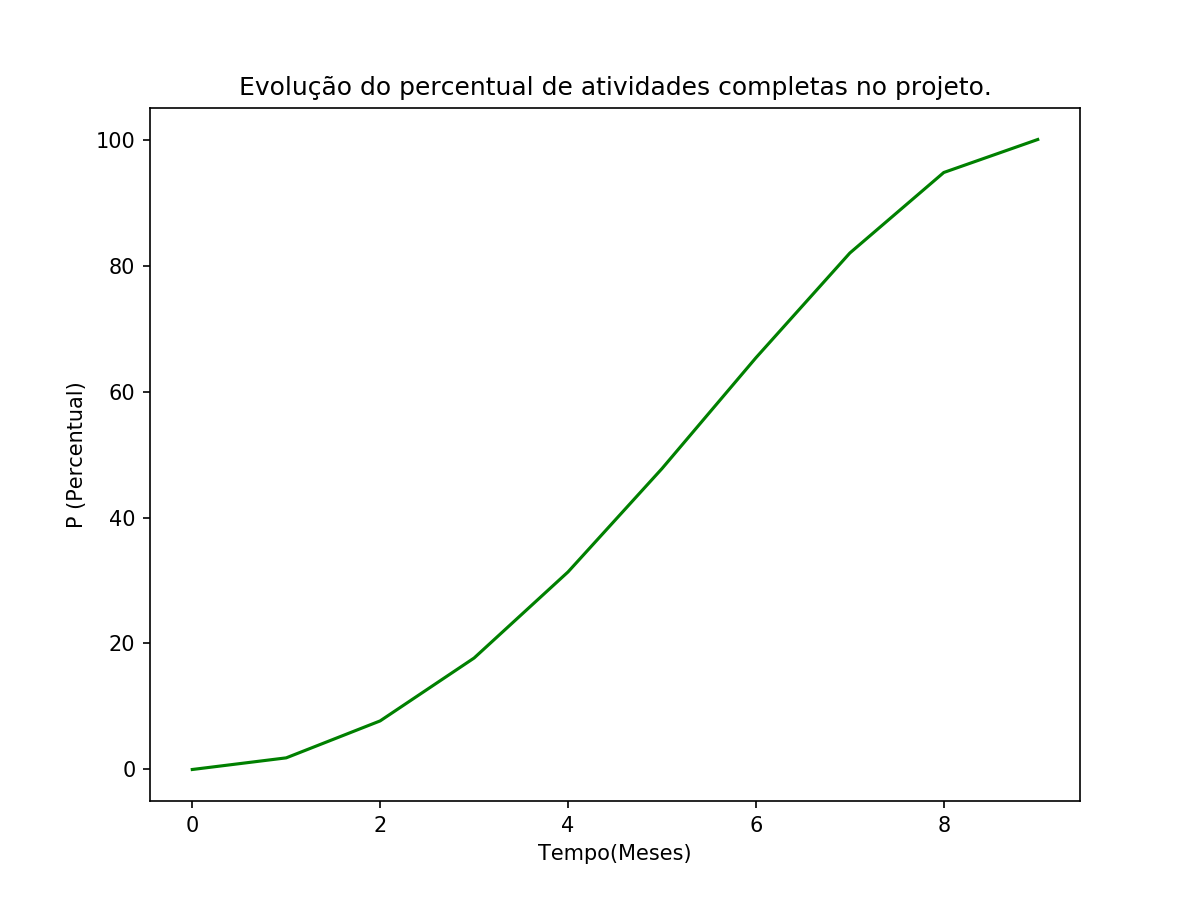
\includegraphics[scale=0.9]{empresa1_p.png}
                \caption{Percentual da Atividade do Projeto 1}
                \label{empresa1_p}
            \end{figure}
            
                \begin{figure}[H]
                \centering
                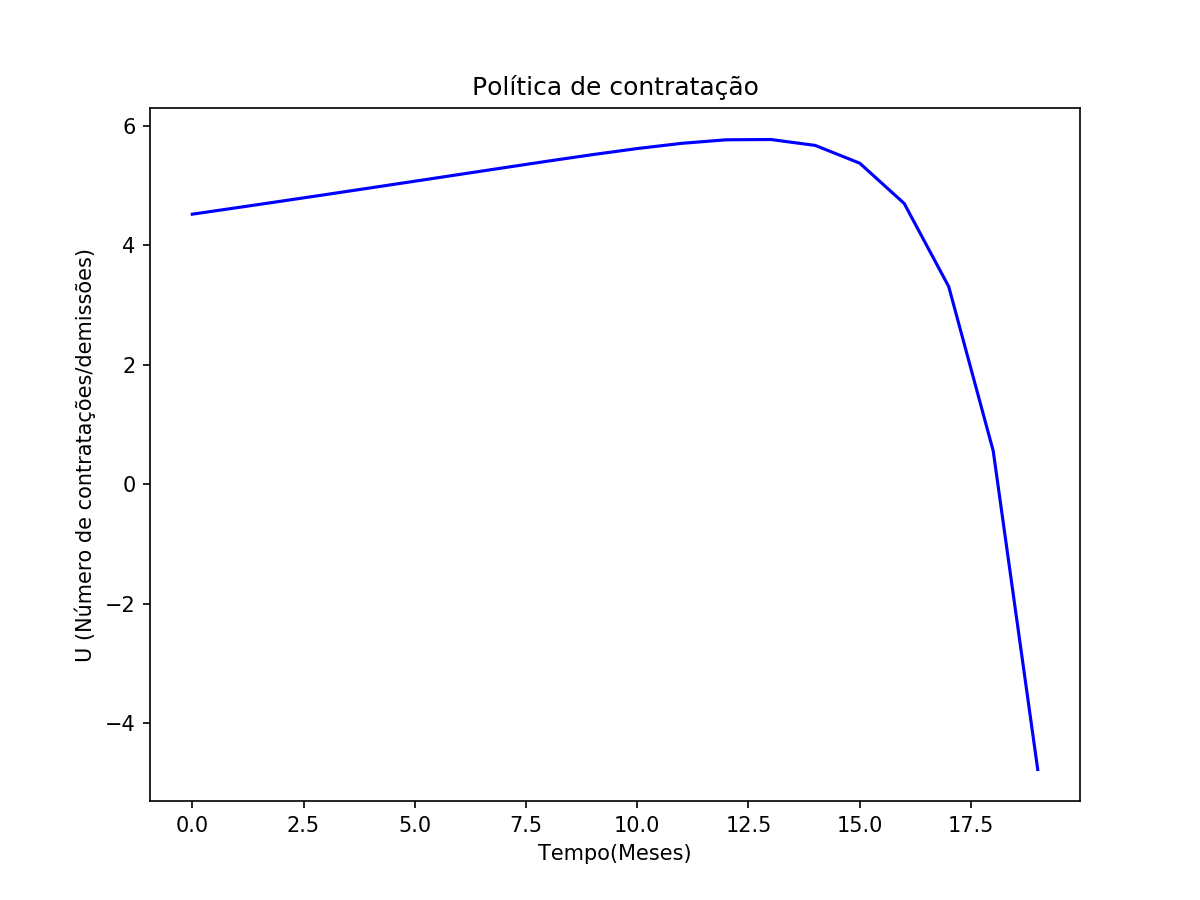
\includegraphics[scale=0.9]{empresa2_u.png}
                \caption{Número de Contratações do Projeto 2}
                \label{empresa2_u}
            \end{figure}
            
            \begin{figure}[H]
                \centering
                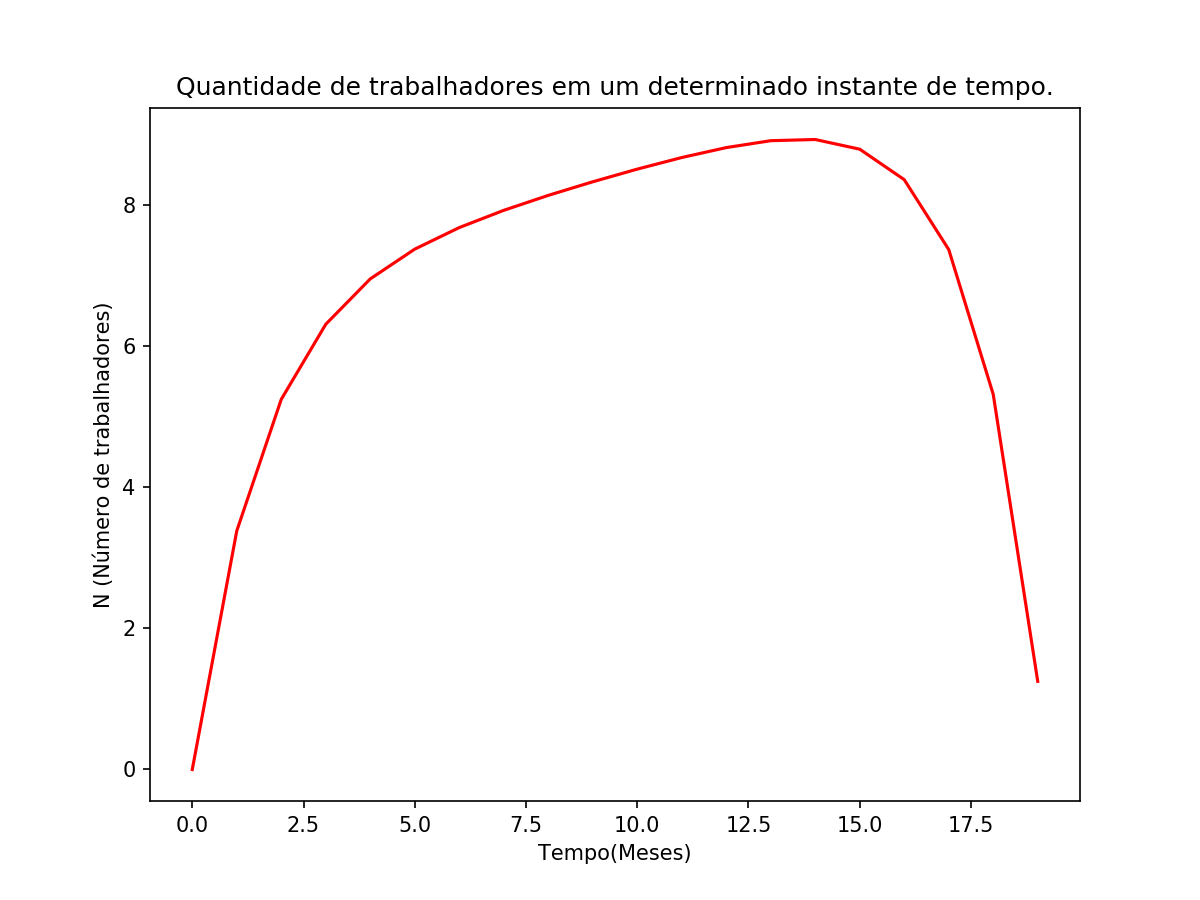
\includegraphics[scale=0.9]{empresa2_n.png}
                \caption{Número de Funcionários do Projeto 2}
                \label{empresa2_n}
            \end{figure}
            
            \begin{figure}[H]
                \centering
                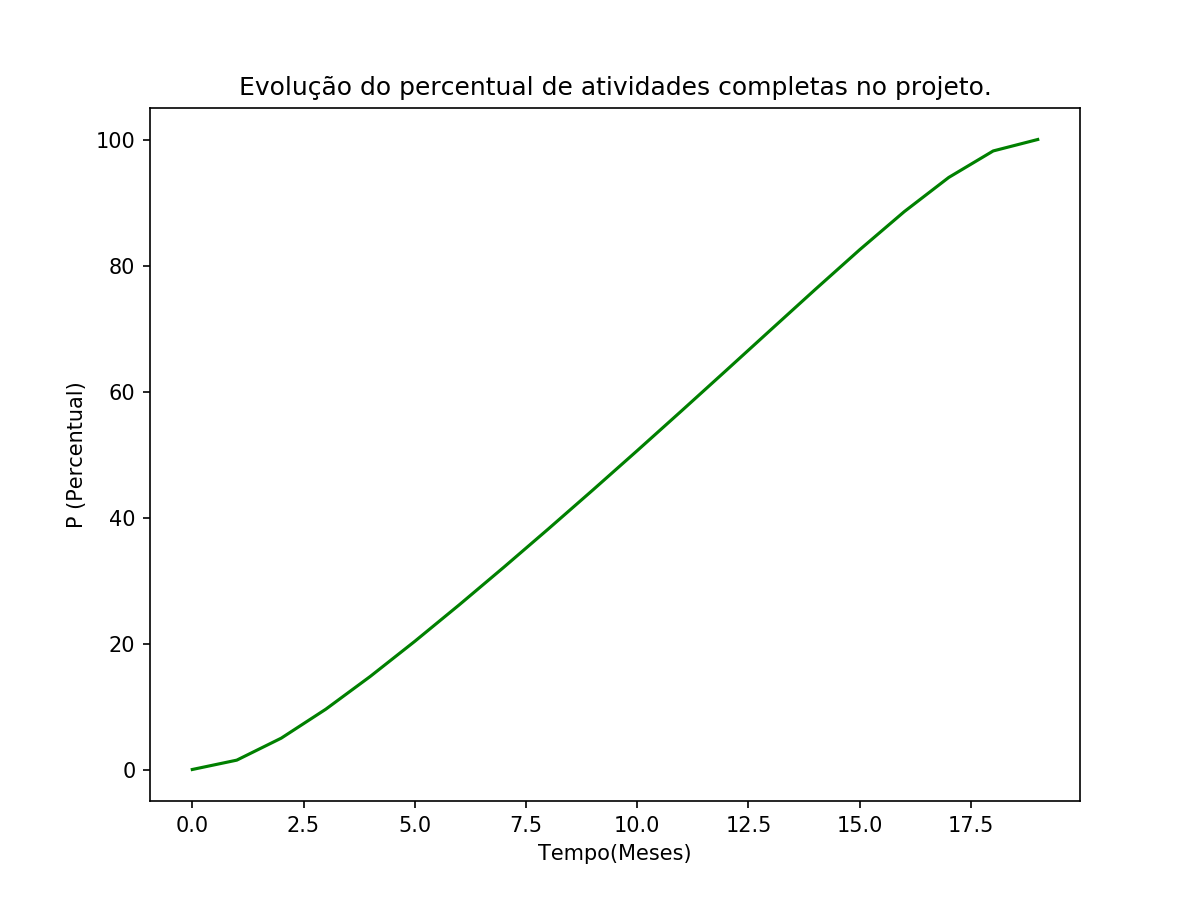
\includegraphics[scale=0.9]{empresa2_p.png}
                \caption{Percentual da Atividade do Projeto 2}
                \label{empresa2_p}
            \end{figure}
            
                \begin{figure}[H]
                \centering
                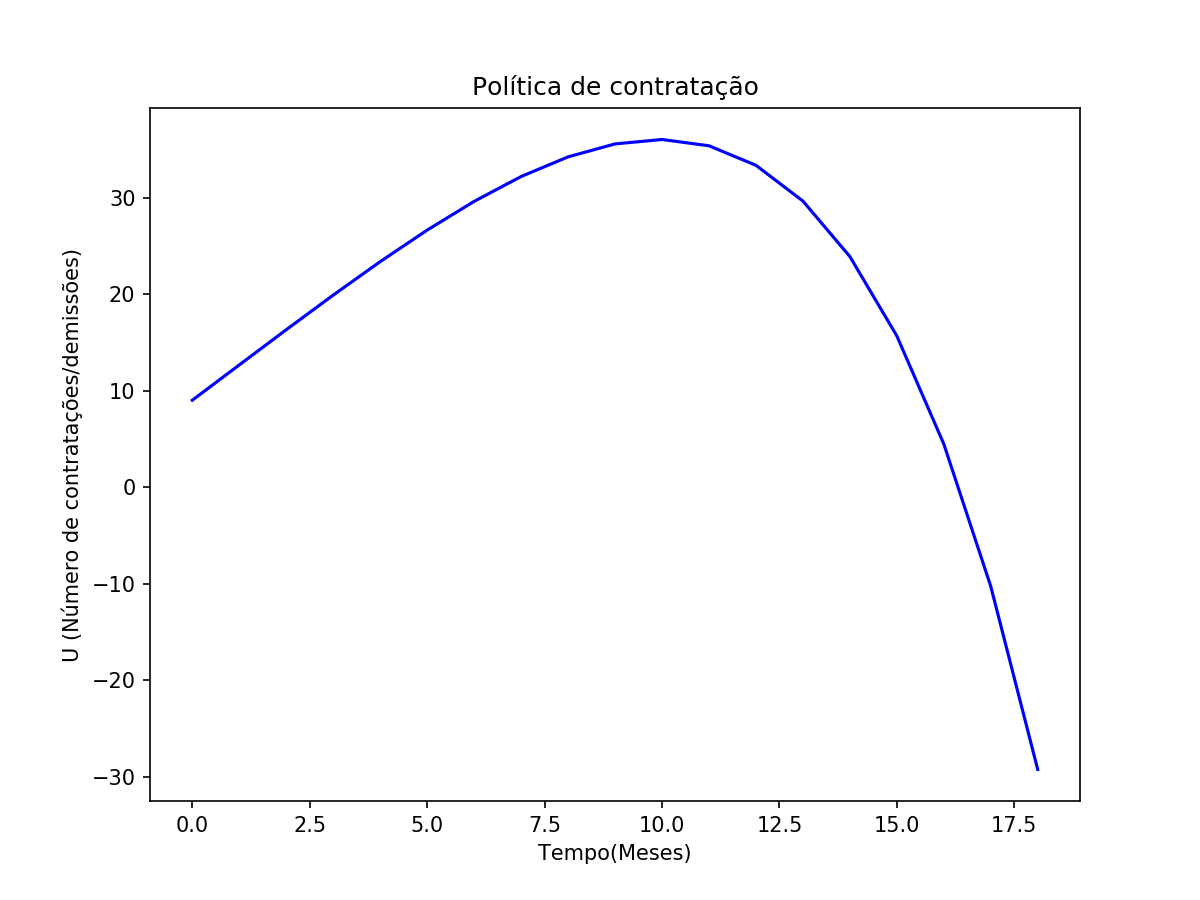
\includegraphics[scale=0.9]{empresa3_u.png}
                \caption{Número de Contratações do Projeto 3}
                \label{empresa3_u}
            \end{figure}
            
            \begin{figure}[H]
                \centering
                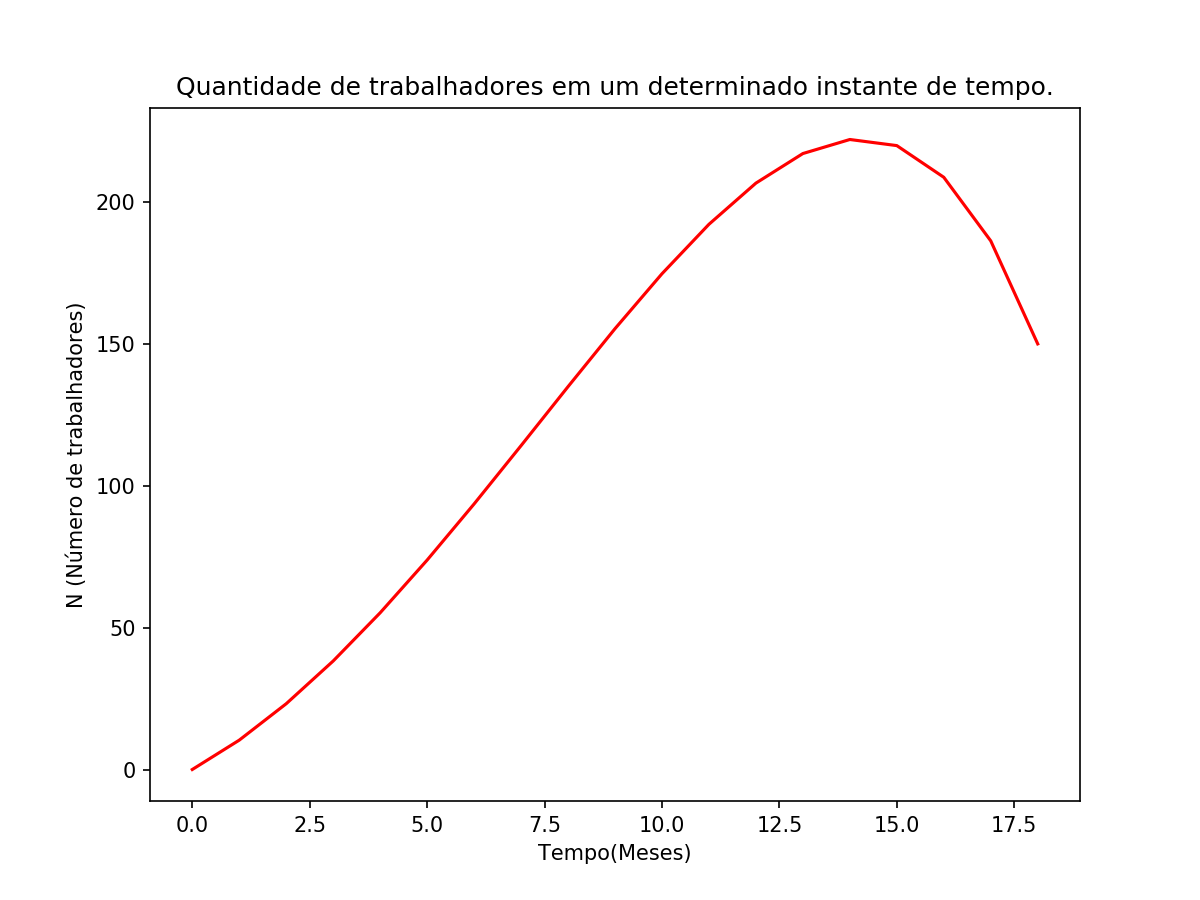
\includegraphics[scale=0.9]{empresa3_n.png}
                \caption{Número de Funcionários do Projeto 3}
                \label{empresa3_n}
            \end{figure}
            
            \begin{figure}[H]
                \centering
                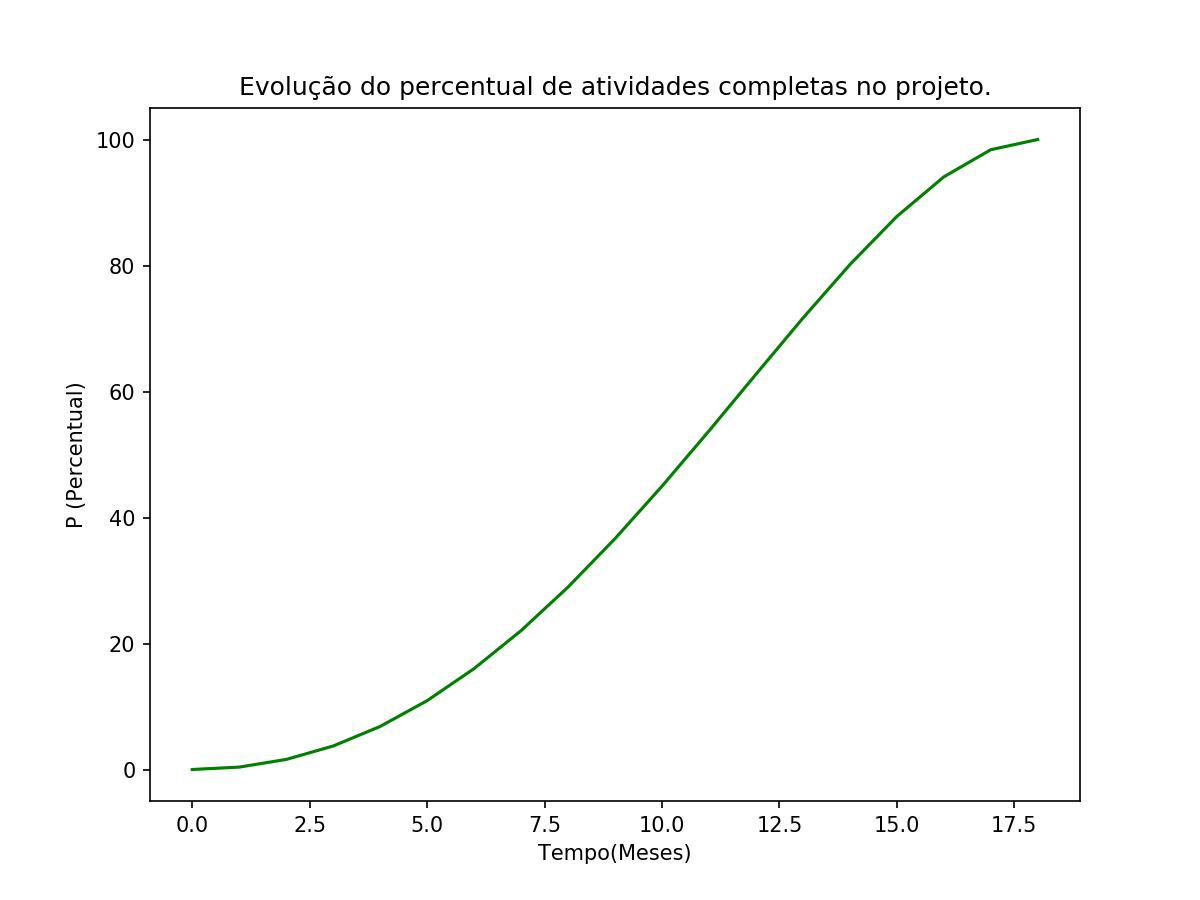
\includegraphics[scale=0.9]{empresa3_p.png}
                \caption{Percentual da Atividade do Projeto 3}
                \label{empresa3_p}
            \end{figure}
            
            \pagebreak
            \begin{python}
import matplotlib.pyplot as plt
import math
import numpy as np


#Valores utilizados para as constantes alfa,mi,gama,beta,teta,tau .

'''PARAMETERS
α Change requests Increasing of project
μ Resignment Fair dismissal Labor accident Diseases
γ Productivity
β Cost with remunerations (wages, bonuses, etc.).Cost with social charges.
θ Cost with hiring/firing Cost with training/adaptation/transfer
τ Ending time
'''
alpha,mi,gama,beta,teta,tau=0.02,0.5,0.01,1500,550,30
tempo=tau + 1


#achando os valores das contantes de integração

a=1/(4*teta*mi)
b= -gama/((2*teta)*(alpha**2-mi**2))
c = gama/((4*teta*mi)*(alpha+mi))
d=gama/(alpha-mi)
f=-(gama**2)/(4*teta*alpha*(alpha**2-mi**2))
g= math.exp(mi*tau)/(4*teta*mi)
h=math.exp(-mi*tau)
i=-gama*math.exp(alpha*tau)/(2*teta*(alpha**2-mi**2))
j= gama*math.exp(mi*tau)/(4*teta*mi*(alpha+mi))
l= gama*math.exp(-mi*tau)/(alpha-mi)
m= math.exp(-alpha*tau)
n= -gama**2*math.exp(alpha*tau)/(4*teta*alpha*(alpha**2-mi**2))
u=beta/(2*teta*mi**2)
v=gama*beta/(2*teta*alpha*mi**2)
x=(alpha/gama) + beta/(2*teta*mi**2)
z= 1 + gama*beta/(2*teta*alpha*mi**2)



A=((m*v -z)*(a*h - g) + (u*g - x*a)*(d*m - l) + (u*h - x)*(j-c*m))/((m*f - n
)*(a*h - g) + (b*g - i*a)*(d*m-l) +(b*h-i)*(j-c*m))
B=(i-b*h)*A/(a*h-g) -(x-u*h)/(a*h-g)
C=u-b*A -a*B
D=(v-u*d) -(f - b*d)*A -(c- a*d)*B




U,N,P=[],[],[]
for t in range(tempo):
    U.append(-beta/(2*teta*mi)-(gama*A*math.exp(alpha*t)/(2*teta*(alpha-mi)))+(B*math.exp(mi*t))/(2*teta))
    N.append(-beta/(2*teta*(mi**2))-(gama*A*math.exp(alpha*t))/(2*teta*((alpha**2)-(mi**2)))+(B*math.exp(mi*t)/(4*teta*mi))+C*math.exp(-mi*t))
    P.append(-gama*beta/(2*teta*alpha*mi**2)-(gama**2*A*math.exp(alpha*t))/(4*teta*alpha*(alpha**2-mi**2))+
        (gama*B*math.exp(mi*t))/(4*teta*mi*(alpha + mi))+(gama*C*math.exp(-mi*t))/(alpha-mi)+D*math.exp(-alpha*t))



plt.figure(figsize=(8, 6), dpi=150)
plt.plot(list(range(tempo)), N,'r')
plt.title("Quantidade de trabalhadores em um determinado instante de tempo.")
plt.xlabel("Tempo")
plt.ylabel("N (Número de trabalhadores)")
plt.savefig("grafico_n.png")

plt.figure(figsize=(8, 6), dpi=150)
plt.plot(list(range(tempo)), U,'b')
plt.title("Política de contratação")
plt.xlabel("Tempo")
plt.ylabel("U (Número de contratações/demissões)")
plt.savefig("grafico_u.png")

plt.figure(figsize=(8, 6), dpi=150)
plt.plot(list(range(tempo)), [i*100 for i in P],'g')
plt.title("Evolução do percentual de atividades completas no projeto.")
plt.xlabel("Tempo")
plt.ylabel("P (Percentual)")
plt.savefig("grafico_p.png")

            \end{python}
            
            \chapter[Conclusão]{\hyperlink{toc}{Conclusão}}
            Em suma, pode-se perceber que ao utilizar a modelagem matemática do método de otimização de recursos humanos, o comportamento do percentual de atividades são similares aos três casos simulados, \textbf{o que indica...}  .
            Para garantir a confiabilidade da projeção obtida pelo método, é necessário que um estudo minucioso do histórico da empresa seja feito, para que cada parâmetro que informe o comportamento da equação realmente reflita o funcionamento da empresa.
            
            
           
        
           %referencias bibliograficas do projeto
        \begin{thebibliography}{9}
            \bibitem{guilherme} 
                C, Guilherme. 
            \textit{Optimum Measurement of Human Resources in Projects.}
                Recife
        
        \end{thebibliography}


	        
\end{document}